\documentclass{thesisclass}

%% -------------------------------
%% |    IM Thesis Template       |
%% -------------------------------
%% Further additions by: Philipp Stroehle, IM, 2013 
%% philipp.stroehle "at" kit.edu

%% Notes:
%% Language switch after \begin{document}

% Based on thesisclass.cls of Timo Rohrberg, 2009
% ----------------------------------------------------------------
% Thesis - Main document
% ----------------------------------------------------------------

% Select your thesis language here:
\usepackage[english]{babel}
%\usepackage[ngerman]{babel}


%% ---------------------------------
%% |      Additional packages      |
%% ---------------------------------
%% 

\usepackage{graphicx}
%http://en.wikibooks.org/wiki/LaTeX/Importing_Graphics#Graphics_storage
\DeclareGraphicsExtensions{.pdf,.png,.jpg}
\graphicspath{{./figures/}} %Use curly braces for each path to add and don't
% forget trailing slash '/'
% \usepackage{epstopdf} %Nice to automatically convert eps figures to pdf
% format  (from inkscape, etc)
\usepackage[natbibapa]{apacite}
\usepackage{booktabs}
\usepackage{wrapfig}

%% ---------------------------------
%% | Needed for the List of Abbreviations |
%% ---------------------------------
\usepackage{nomencl}
\renewcommand{\nomname}{List of Abbreviations}
% Punkte zw. Abkürzung und Erklärung
\setlength{\nomlabelwidth}{.32\hsize}%.32\hsize bezieht sich auf die Punkte zwischen Abkürzung und Erklärung -> je größer die Zahl, desto mehr %Punkte
\renewcommand{\nomlabel}[1]{#1 \dotfill}
% Zeilenabstände verkleinern
\setlength{\nomitemsep}{-\parsep}
\makenomenclature
\usepackage[normalem]{ulem}
\newcommand{\markup}[1]{\uline{#1}}


%% ---------------------------------
%% | Information about the thesis  |
%% ---------------------------------

% uncomment one of the following, according to your thesis
%\newcommand{\mytype}{\iflanguage{english}{Bachelor Thesis}{Bachelorarbeit}} 
%\newcommand{\mytype}{\iflanguage{english}{Master's Thesis}{Masterarbeit}} 
\newcommand{\mytype}{\iflanguage{english}{Seminar Thesis}{Seminararbeit}} 

\newcommand{\myname}{Nico Rausch\\Richard Tran\\Giorgio Groß}
\newcommand{\matricle}{1856484 - 1835121 - 1938927}
\newcommand{\mytitle}{\iflanguage{english}{Hack\&Slash: Gesture Recognition for Dashboards}{Titel der Arbeit}}
\newcommand{\myinstitute}{\iflanguage{english}
{Institute of Information Systems and Marketing (IISM) \\
Information \& Market Engineering}
{Institut für Informationswirtschaft und Marketing (IISM) \\
Information \& Market Engineering}}

\newcommand{\reviewerone}{Prof. Dr. Alexander Mädche}
\newcommand{\reviewertwo}{}
\newcommand{\advisor}{Eric Pescera (TECO)}
\newcommand{\advisortwo}{}

\newcommand{\timestart}{\iflanguage{english}{20. July 2017}{XX. Monat 20XX}}
\newcommand{\timeend}{\iflanguage{english}{20th of July 2017}{XX. Monat 20XX}}
\newcommand{\submissiontime}{20. 07. 2017}

%% -------------------------------
%% |  Information for PDF file   |
%% -------------------------------
%% IM: Auto-Fill this information
\hypersetup{
 pdfauthor={\myname},
 pdftitle={\mytitle},
 pdfsubject={\mytype},
 pdfkeywords={\mytype}
}

%% ---------------------------------
%% | ToDo Marker - only for draft! |
%% ---------------------------------
% Remove this section for final version!
\setlength{\marginparwidth}{20mm}

\newcommand{\margtodo}
{\marginpar{\textbf{\colorbox{yellow}{ToDo}}}{}}


\newcommand{\todo}[1]{\margtodo{}\colorbox{yellow}{#1}}


%% --------------------------------
%% | Old Marker - only for draft! |
%% --------------------------------
% Remove this section for final version!
\newenvironment{deprecated}
{\begin{color}{gray}}
{\end{color}}


%% --------------------------------
%% | Settings for word separation |
%% --------------------------------
% Help for separation:
% In german package the following hints are additionally available:
% "- = Additional separation
% "| = Suppress ligation and possible separation (e.g. Schaf"|fell)
% "~ = Hyphenation without separation (e.g. bergauf und "~ab)
% "= = Hyphenation with separation before and after
% "" = Separation without a hyphenation (e.g. und/""oder)

% Describe separation hints here:
\hyphenation{
% Pro-to-koll-in-stan-zen
% Ma-na-ge-ment  Netz-werk-ele-men-ten
% Netz-werk Netz-werk-re-ser-vie-rung
% Netz-werk-adap-ter Fein-ju-stier-ung
% Da-ten-strom-spe-zi-fi-ka-tion Pa-ket-rumpf
% Kon-troll-in-stanz
}


%% ------------------------
%% |    Including files   |
%% ------------------------
% Only files listed here will be included!
% Userful command for partially translating the document (for bug-fixing e.g.)
\includeonly{%
titlepage,
text/abbreviations,
text/introduction,
text/content,
text/evaluation,
text/conclusion,
text/declaration,
text/appendix
}

%%%%%%%%%%%%%%%%%%%%%%%%%%%%%%%%%
%% Here, main documents begins %%
%%%%%%%%%%%%%%%%%%%%%%%%%%%%%%%%%
\begin{document}

\frontmatter
\pagenumbering{roman}
%% titlepage.tex
%%

% coordinates for the bg shape on the titlepage
\newcommand{\diameter}{20}
\newcommand{\xone}{-15}
\newcommand{\xtwo}{160}
\newcommand{\yone}{15}
\newcommand{\ytwo}{-253}

\begin{titlepage}
% bg shape
\begin{tikzpicture}[overlay]
\draw[color=gray]  
 		 (\xone mm, \yone mm)
  -- (\xtwo mm, \yone mm)
 arc (90:0:\diameter pt) 
  -- (\xtwo mm + \diameter pt , \ytwo mm) 
	-- (\xone mm + \diameter pt , \ytwo mm)
 arc (270:180:\diameter pt)
	-- (\xone mm, \yone mm);
\end{tikzpicture}
	\begin{textblock}{10}[0,0](4,2.5)
		\iflanguage{english}
			{
\includegraphics[width=.3\textwidth]{logos/KITLogo_EN_RGB.pdf}}
			{
\includegraphics[width=.3\textwidth]{logos/KITLogo_DE_RGB.pdf}}		
	\end{textblock}
	\begin{textblock}{10}[0,0](10,2.5)
		
\includegraphics[width=.6\textwidth]{logos/IISMLogo_RGB.pdf}
	\end{textblock}
	\changefont{ppl}{m}{n}	% helvetica	(phv), % IM Style: palatino (ppl) 
	\vspace*{2.5cm}
	\begin{center}
		\Huge{\mytitle}
		\vspace*{1.5cm}\\
		\Large{
			\iflanguage{english}{\mytype}			
								{\mytype}
		}\\
		\vspace*{1cm}
		\huge{\myname}\\
			\Large{\matricle}\\
		\vspace*{1cm}
		\Large{
			\iflanguage{english}{At the Department of Economics and Management}			
							    {An der Fakult\"at f\"ur Wirtschaftswissenschaften}
			\\
			\myinstitute
		}
	\end{center}
	\vspace*{2cm}
\Large{
\begin{center}
\begin{tabular}[ht]{l c l}
  % Gutachter sind die Professoren, die die Arbeit bewerten. 
  %\iflanguage{english}{Reviewer}{Erstgutachter}: & \hfill  & \reviewerone\\
  %\iflanguage{english}{Reviewer}{Gutachter}: & \hfill  & \reviewerone\\
  %\iflanguage{english}{Second reviewer}{Zweitgutachter}: & \hfill  & \reviewertwo\\
  \iflanguage{english}{Advisor}{Betreuender Assistent}: & \hfill  & \advisor\\
  % \iflanguage{english}{Second advisor}{Zweiter betreuender Mitarbeiter}: & \hfill  & \advisortwo\\
  % IM: No second advisor
  % Der zweite betreuende Mitarbeiter kann weggelassen werden. 
\end{tabular}
\end{center}
}


\vspace{3cm}
\begin{center}
\large{\timeend}
% \iflanguage{english}{Duration:}{Bearbeitungszeit:} \timestart \hspace*{0.25cm}
% -- \hspace*{0.25cm} 
% \timeend}
\end{center}


\begin{textblock}{10}[0,0](4,16.8)
\tiny{ 
	\iflanguage{english}
		{KIT -- University of the State of Baden-Wuerttemberg and National Laboratory of the Helmholtz Association}
		{KIT -- Universit\"at des Landes Baden-W\"urttemberg und nationales Forschungszentrum der Helmholtz-Gesellschaft}
}
\end{textblock}

\begin{textblock}{10}[0,0](14,16.75)
\large{
	\textbf{www.kit.edu} 
}
\end{textblock}

\end{titlepage}

% IM Style: No additional blank page
% \blankpage


%% -------------------
%% |   Directories   |
%% -------------------
\tableofcontents
% IM Style: No additional blank page
% \blankpaage

% Do not include a list of figures, list of tables and list of abbreviations, if the work is a seminar thesis
\iflanguage{english}{
\ifthenelse{\equal{\mytype}{Seminar Thesis}}
{}
{
\listoffigures \addcontentsline{toc}{chapter}{List of Figures} 
\listoftables  \addcontentsline{toc}{chapter}{List of Tables} 
\printnomenclature   \addcontentsline{toc}{chapter}{List of Abbreviations} 
}
}
{
\ifthenelse{\equal{\mytype}{Seminararbeit}}
{}
{
\listoffigures \addcontentsline{toc}{chapter}{Abbildungsverzeichnis} 
\listoftables \addcontentsline{toc}{chapter}{Tabellenverzeichnis} 
\printnomenclature \addcontentsline{toc}{chapter}{Abkürzungsverzeichnis}
}
}

% Execute this command for index creation, i.e., for abbreviations by the nomencl package
% makeindex thesis.nlo -s nomencl.ist -o thesis.nls



%\printnomenclature



%% -----------------
%% |   Main part   |
%% -----------------
\mainmatter
\pagenumbering{arabic}
%% introduction.tex
%%

%% ==============================
\chapter{Introduction}
\label{ch:Introduction}
%% ==============================

Nowadays gesture recognition has achieved a high usage and meaning, especially for medical purposes and industrial production processes.
These new technologies are available not only for industrial purposes, but also for the mass market, for which devices like the Xbox Kinect or the Wii Remote set the basis a few years ago.
Until now, many research groups (\cite{vision1},\cite{vision3},\cite{vision2}) have already worked on technologies which enable the user to control computers with gestures.
Most of these devices work vision-based, i.e. with cameras which recognize the visual changes caused by body movement and translate them into computer commands.
These applications have the disadvantage that the user cannot move freely in the room, since he is bounded to the space captured by the camera in order to transmit the commands properly.
This can be impractical for specific situations, e.g. presentations, when flexibility is needed considering the movement in the room.

Furthermore, there are also several technologies which track the physical data of the movement with the help of sensors (accelerometer, gyroscope, etc.) to recognize a gesture.
These can be used independently from the location of the user in the room, but often demands expensive equipment, for instance a data glove.
In order to develop a cheap and accurate sensor based gesture recognition device, different approaches use data from an accelerometer to classify gestures.
These show a high accuracy, but are limited in the number of different identifiable gestures due to the less data.

In our work, we used the “Thunderboard React”, which is a development platform with several sensors including an accelerometer and a gyroscope.
We examined, how well such a sensor platform is suited for gesture recognition and how it enhances dashboard user experiences.
We did this by calculating “features” like the maximal acceleration from the collected data and classified these with different machine learning approaches.
Overall, we established to recognize 4 different gestures with an expectancy accuracy of 95\%.
Furthermore, we created a dashboard to test the usability of our implementation.

%% content.tex
%%

%% ==============
\chapter{Related Work}
\label{ch:Related Work}
%% ==============

Gesture recognition with wearable devices has been an important research topic over the years. 
There have been a lot of works which used accelerometer-based devices, such as a Wii remote or a data glove. 
Xu, Zhou and Li experimented with classifying seven hand gestures using the sign sequence of the gesture acceleration as the main feature (\cite{xu}). 
They tried three different recognition algorithms in order to find the most suitable one. 
The movement data was gathered using MEMS 3-axis accelerometer with a Bluetooth connection to a PC. 
With a dataset of overall 628 samples they achieved an average recognition accuracy of 95.6\% and they concluded, that in this experiment the recognition algorithm based on sign sequence and template matching was the most accurate algorithm. 
Liu also used template matching in order to classify accelerometer data (\cite{liu}). 
In their experiments, they utilized the three-axis accelerometer from the Wii remote as input device for their classifier. 
They evaluated a large gesture library with over 4000 samples for eight gesture patterns and their results show an overall 98.6\% accuracy and a recognition delay of only 300 ms. 
Kim, Thang and Kim used several accelerometers, with which they created a data glove that was connected via Bluetooth with the PC (\cite{kim}). 
They performed simple hand gesture recognition by considering a 10-point moving average of the acceleration with which they could achieve a recognition accuracy of 100\% for only three distinct hand gestures. 

Further work has been done focusing on which machine learning algorithm performs best regarding gesture recognition. 
Belgioioso examined acceleration data collected from an iPod Touch and a HTC-Explorer smartphone. 
They experimented based on a dataset of overall 550 samples for four types of gestures and tested classification approaches such as Support Vector Machine (SVM), Relevance Vector Machine (RVM), Sparse Bayesian Learning (SBL) or k-Nearest Neighbor (kNN) (\cite{belgioioso}). 
For feature extraction, they employed a Principal Component Analysis which is an approach to reduce the dimensionality of a data set consisting of many variables correlated with each other. 
The work concluded that SVM has proved to be the approach with the highest accuracy in recognizing gestures, while SBL based approaches showed comparable classification performances with less computational cost required.
To the best of our knowledge, this work presents the first gesture recognition study using the Thunderboard react.


%% ==============
\chapter{System Design}
\label{ch:SystemDesign}
%% ==============

In order to maximize reusability of code we decided to split the app into the six main components shown below. As you can see, our project consists of two individual parts, the recorder app and the recognizer app, sharing two helper modules, labeled Input and Connector. We implemented a core module for each part which is responsible to coordinate data streams and event responses. As such, the core modules instantiate their helper modules and use their interfaces to communicate with them. It is also worth knowing that some modules are divided into multiple files which are documented directly in our code.

%% ===========================
\section{Components}
\label{ch:SystemDesign:sec:Components}
%% ===========================

\begin{figure}[htp]
\begin{center}
  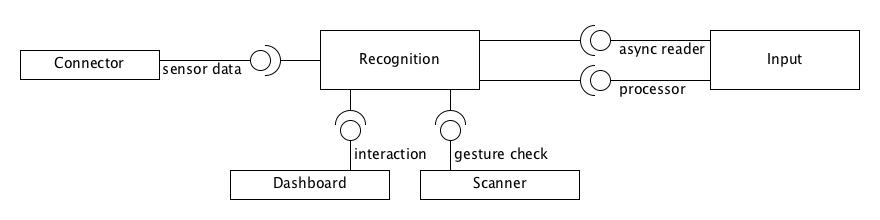
\includegraphics[width = \textwidth]{Component_diagram_recognizer.jpg}
\caption{Recognizer App}
\end{center}
\end{figure} 

\begin{figure}[htp]
\begin{center}
  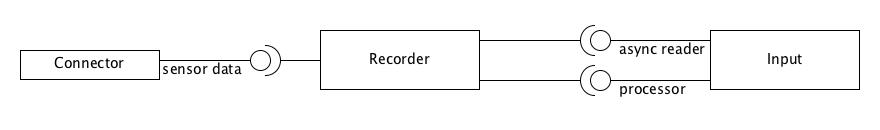
\includegraphics[width = \textwidth]{Component_diagram_recorder.jpg}
\caption{Recoreder App}
\end{center}
\end{figure} 

\newpage

%% ===========================
\subsection{Connector}
\label{ch:SystemDesign:sec:Components:sub:Connector}
%% ===========================
\setlength\intextsep{0pt}
\begin{wrapfigure}{R}{0.5\textwidth}
\centering
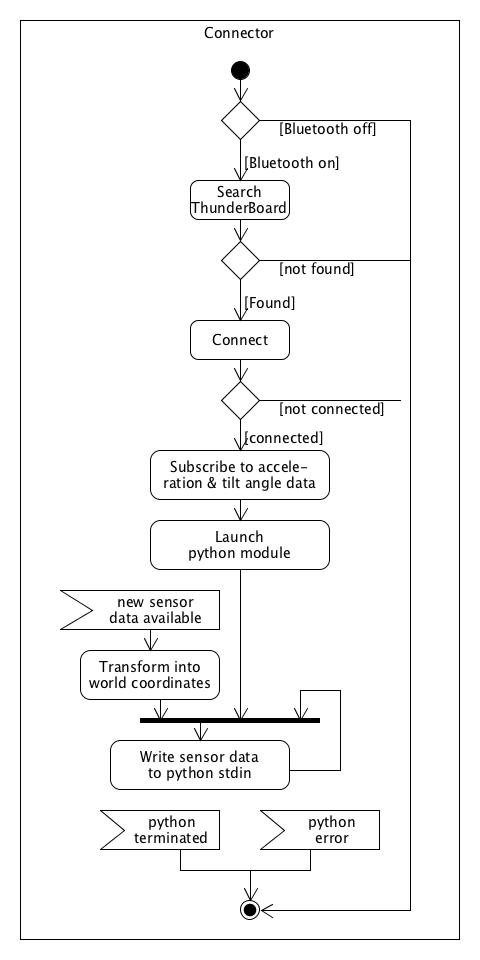
\includegraphics[width=0.5\textwidth]{Connector_flow.jpg}
\caption{Establishing the connection to the Thunderboard React}\label{fig:flow_chart}
\end{wrapfigure}

As we ran into several issues trying to connect the Thunderboard React using Python we implemented the connector in JavaScript and used NodeJS libraries for interfacing the bluetooth device. To launch the recorder or recognizer app you need to launch the connector and pass it the path to the desired core module. After launching the connector it performs the steps shown in the flow chart on the right.

\begin{wrapfigure}{R}{0.4\textwidth}
\centering
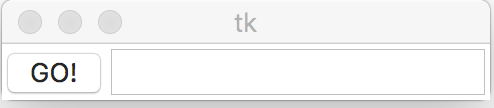
\includegraphics[width=0.4\textwidth]{recorder_screenshot.png}
\caption{Recorder Tool}\label{fig:recorder_screenshot}
\end{wrapfigure}

%% ===========================
\subsection{Input}
\label{ch:SystemDesign:sec:Components:sub:Input}
%% ===========================

The input module starts a new thread upon instantiation to avoid blocking the calling thread. In its new thread it keeps reading the sensor data from stdin, parses it into floating point values and inserts them into a ring buffer. Its interfaces can be used to set up the buffer, to reset the buffer, to insert new data into the buffer or to start recording.  In the latter case, the module finds out when the actual gesture started on its own by comparing the acceleration vector length to a threshold value. As soon as the buffer fills up its content is written to a static CSV file autonomously. The input module never takes action on its own but is still smart enough to perform a full control flow to record a gesture or to maintain the ring buffer.

%% ===========================
\subsection{Recorder}
\label{ch:SystemDesign:sec:Components:sub:Recorder}
%% ===========================

The recorder module provides a simple user interface which is used to specify the gesture you want to record as well as to explicitly start recording. That is done through a button which has to be pressed before each single gesture; we implemented it this way in order to avoid accidentally record a gesture which would pollute our training set. It also is responsible for instantiation and hooking up the input module.

%% ===========================
\subsection{Scanner}
\label{ch:SystemDesign:sec:Components:sub:Scanner}
%% ===========================

The scanner module is only used by the recognition module. It is used for monitoring the ring buffer content and for checking whether a gesture was observed. Thus, it instantiates, trains and maintains the machine learning algorithm used to classify live sensor data. Training includes transforming the recorded raw acceleration and tilt angle data into features and feeding them to the machine learning algorithm. All live sensor data will  also have to be transformed into the same features so that they can be classified. We describe what features are and how we transformed the raw data in the next chapter.
To avoid unnecessary complexity, we included the cross validation used to evaluate the performance of different machine learning algorithms directly into the scanner module. Cross validation includes leave one out, 10-fold cross validation and 25-fold cross validation and is performed during instantiation.


%% ===========================
\subsection{Recognition}
\label{ch:SystemDesign:sec:Components:sub:Recognition}
%% ===========================

The recognition module used in the recognizer app is responsible to instantiate and hooking up the input module. It also instantiates the dashboard and implements the logic required to notify it about a recognized gesture.

%% ===========================
\chapter{Data Collection \& Manipulation}
\label{ch:DataCollection}
%% ===========================

Working  with  machine  learning  algorithms  requires  certain  actions  in  order  to choose, prepare and classify data streams.
Choosing the right data is the key decision in order to be able to train the  algorithm properly.
In addition to this  step, preparing data and transforming it into “features” is equally important. 

%% ===========================
\section{Data Collection}
\label{ch:DataCollection:sec:DataCollection}
%% ===========================

To  define  which  data  will  be  collected  we  had  to  think  about  which  kind  of gestures  we  will  want  to  recognize.
Attaching  the  sensors  to  the  back  of  our  hand enables us to observe acceleration data  for x,  y, and z axis  as well  as tilt  angles  alpha, beta and gamma.
We thought about attaching a magnet to our thumb so that we can use the hall-sensor as well,  but we decided to leave this  for  further research.
The collected acceleration and tilt angle data can later be used to distinguish gestures from each other.
For collecting all the data we need, we use our recorder system, which reads data from the ThunderBoard by using our connector module and giving us the possibility to tag the recorded gesture with an ID.
The ThunderBoard is therefor attached to the back of the right hand.
To avoid recording and scanning data observed during normal gesticulation we require the acceleration vector length of each gesture to exceed a certain threshold.
In our code we set this treshold to 1.2 G.
As soon as the treshold is exceeded, our recorder saves the next four data points and the specified gesture ID as row in a CSV file.
All in all, our team recorded 120 data sets per gesture, so 480 data sets overall.
Because the recorded data is really slow to progress we decided to stop at this point, although we initially wanted external people to record some data for us.

%% ===========================
\section{Gestures}
\label{ch:DataCollection:sec:Gestures}
%% ===========================

Really early in development, we thought about what gestures we can detect and what gestures are useful for us.
We came up with many ideas, but the first two gestures we implemented were the two most intuitive gestures for us: Swipe Left and Swipe Right.
For easy recognition of the gesture, we decided to put rules on the execution of these gestures.
A \glqq swipe left\grqq{} gesture consists of a very fast movement of the active hand to the left, followed by a slow movement back to the initial position.
Both movements should not include a big tilt of the board.
The \glqq swipe right\grqq{} gesture is just the same, but with switched directions.
By adding those rules we increased the success of recognition hugely.
As a consequence, we removed the first data sets we recorded, without those rules, from the CSV.
After a few weeks we reached a great success rate on the left and right swipes, so we added additional swipes \glqq Up\grqq{} and \glqq Down\grqq{} and a punch gesture.
The punch gesture is executed like a normal punch with the fist.
Since the \glqq Swipe Down\grqq{} and the punch were often confound, we decided to exclude the \glqq Swipe Down\grqq -Gesture from our work.

%% ===========================
\section{Feature Design}
\label{ch:DataCollection:sec:FeatureDesign}
%% ===========================

Before we can train our algorithm, we  have to transform the recorded data into a set  of  features.
Choosing  and  designing  those  features  affects  the  performance  of  the gesture recognition algorithm heavily.

%% ===========================
\subsection{Preprocessing}
\label{ch:DataCollection:sec:FeatureDesign:sub:Preprocessing}
%% ===========================

Standardization,     scaling,     normalization     and     binarization     are     common preprocessing techniques.
Though, as the acceleration vector and tilt angle sizes are key characteristics  to  distinguish  gestures  scaling,  normalization  and  binarization  are  not applicable for our use case. 

%% ===========================
\subsection{Features}
\label{ch:DataCollection:sec:FeatureDesign:sub:Features}
%% ===========================

\begin{figure}
\begin{center}
  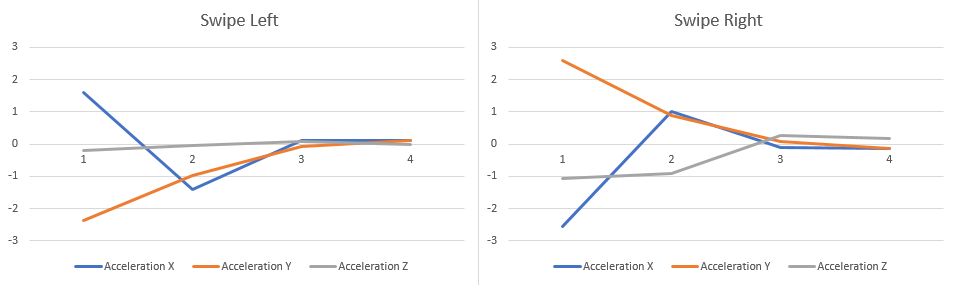
\includegraphics[width = 0.88\textwidth]{data.png}
\caption{Choosing our features by looking at exemplary data points}\label{fig:datamining}
\end{center}
\end{figure} 

We  first  thought  about  using  the  variance  as  a  feature,  but  early  tests  have already revealed  that  the  acceleration  data  often  has  the same variance across all of our tested gestures. We needed to find more useful features, that have different values when we execute different gestures.

The way we thought about this set of features was very intuitive. First, we recorded some gestures that we wanted to implement.
We then created graphs for each of our data sets and looked what is characteristic for them.
In Figure \ref{fig:datamining} for example, we could see that the Swipe Left (Swipe Right) gesture first has a minimum (maximum) on the X-Axis, then a maximum (minimum).
So we decided to use maximum  and  minimum  acceleration  per  axis, because they  differ  widely  across gestures  and  are  worth  adding  to  our  feature  set.

To give our classifier an idea of which minimum/maximum was the first, we put them in the right order, so if we have a maximum first, this will be the first feature and the minimum will become the second feature.
For  instance,  swiping  left  first  shows  a negative  minimum  acceleration, e.g. -1.7G, and then a positive  maximum acceleration, e.g. 1.2G, on the x axis.
We now pick those values out of our buffer and figure out which one was earlier, so we can put them in our feature vector in the right order.
In  this example, we end up with the tuple (-1.7, 1.2).

To include the tilt angles into our feature set, we had to come up with a different approach.
Like for acceleration, not only the variance of the given data was not a good idea either for angles, but also their minimum and maximum values are often equally great across different gestures.
Anyway, taking the minimum and maximum into our feature set increased our precision a little bit, so we continued to use them.

Summing  up  all  angles  led  to non-satisfying  results, because they mostly sum up to a value near zero,  so  we  then thought about  more  features  per  angle:
One  sums  up  the absolute  values  of  negative  angles  and  the  other  one  sums  up  the  absolute values  of  the  positive  angles.

Because the Thunderboard does a permanent recalibration, the absolute angles were not really useful. So, in the next step we decided to use only the differences between two angles in our buffer.
This new approach improved our gesture recognition by about 5\%, as you can see in picture \ref{fig:angle_feature}.

\begin{figure}[htp]
\begin{center}
  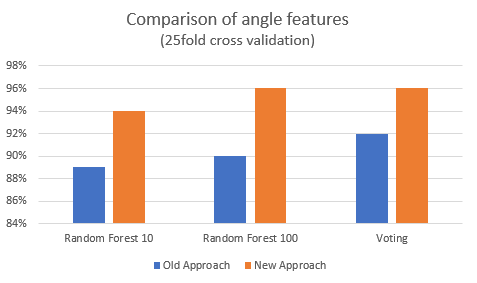
\includegraphics[width=0.5\textwidth]{angle_feature.png}
\caption{Comparison of our old and our new idea}\label{fig:angle_feature}
\end{center}
\end{figure}

\newpage 

%% ===========================
\section{Data Classification}
\label{ch:DataCollection:sec:DataClassification}
%% ===========================

Depending on the underlying training set, each classifier performs a bit different. We tested the K-Neighbors classifier with five and eleven nearest neighbors, Random Forest classifier with 10 and 100 estimators,  Decision Tree classifier, Support Vector Machine and Gaussian Bayes, which is a neural network. We then created a Voting classifier based on two of the best classifiers to push the limits even further. Each classifier was evaluated with leave one out and 10-fold cross validation techniques, the results are summarized in the diagrams below:
\newline
\begin{figure}[H]
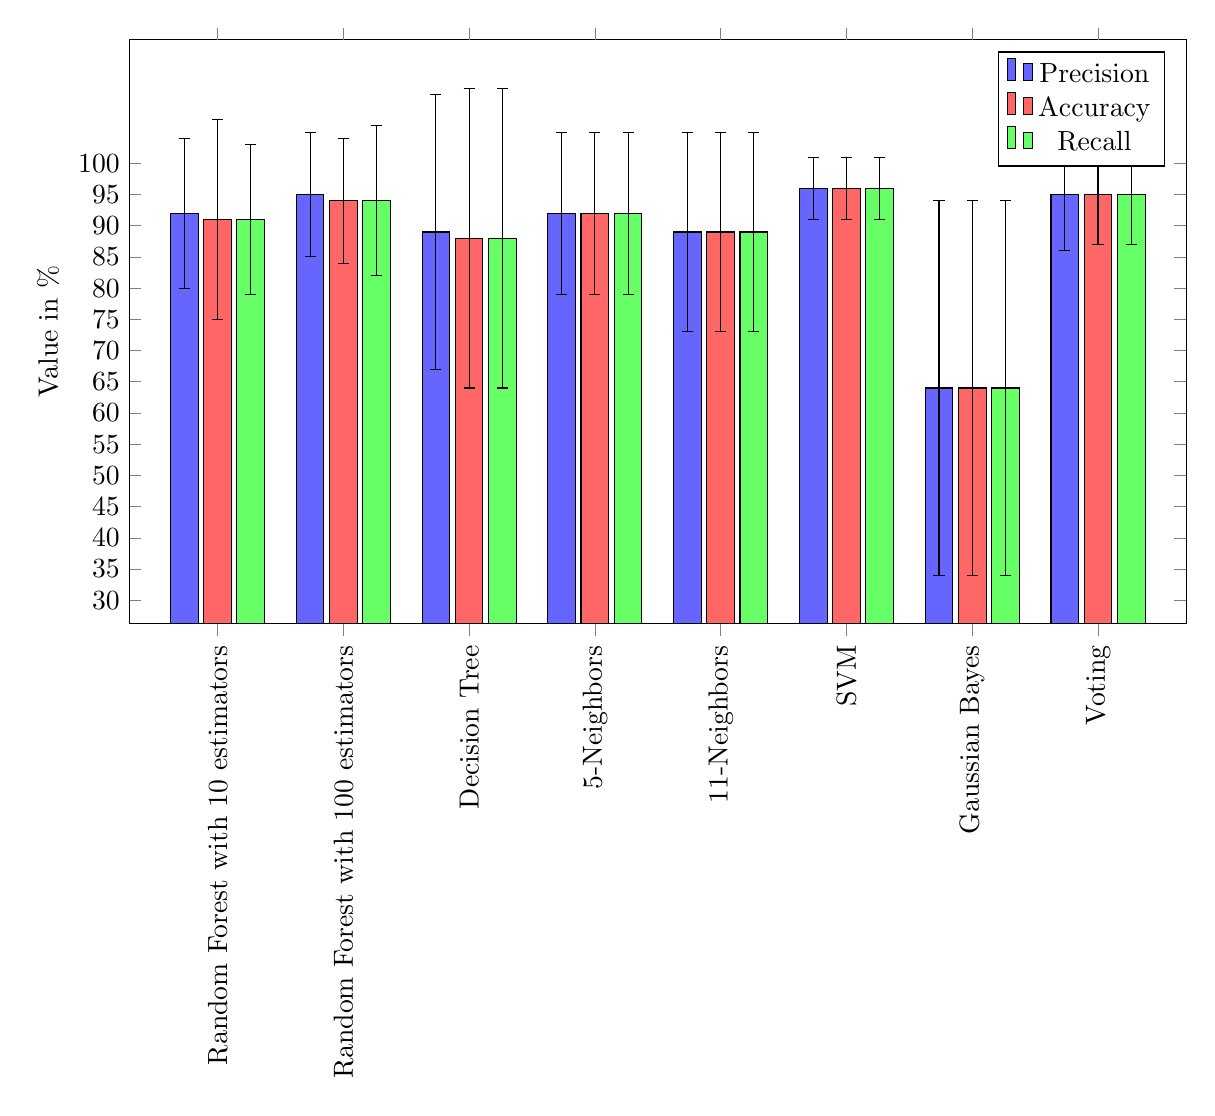
\begin{tikzpicture}
\begin{axis}[
    title = {},
    width=15cm,
    height=9cm,
    xtick=\empty,
    ytick={0,5,...,100},
    ylabel=Value in \%,
    extra x ticks={1,...,8},
    extra x tick labels={%
		Random Forest with 10 estimators,
        Random Forest with 100 estimators,
        Decision Tree,
        5-Neighbors,
        11-Neighbors,
        SVM,
        Gaussian Bayes,
        Voting    
    },
    extra x tick style={
           grid=none,
           tick label style={rotate=90}
           },
    ybar
    ]

\addplot[
    fill=blue!60,
    draw=black,
    point meta=y,
    every node near coord/.style={inner ysep=5pt},
    error bars/.cd,
        y dir=both,
        y explicit
] 
table [y error=error] {
x   y           error    label
1   92   12 1
2   95    10 2
3   89   22 3
4   92   13 4 
5   89    16 5 
6   96   5 6
7   64    30 7 
8   95   9 8
};

\addplot[
    fill=red!60,
    draw=black,
    point meta=y,
    every node near coord/.style={inner ysep=5pt},
    error bars/.cd,
        y dir=both,
        y explicit
] 
table [y error=error] {
x   y           error    label
1   91   16 1
2   94    10 2
3   88   24 3
4   92   13 4 
5   89    16 5 
6   96   5 6
7   64    30 7 
8   95   8 8
};

\addplot[
    fill=green!60,
    draw=black,
    point meta=y,
    every node near coord/.style={inner ysep=5pt},
    error bars/.cd,
        y dir=both,
        y explicit
] 
table [y error=error] {
x   y           error    label
1   91   12 1
2   94    12 2
3   88   24 3
4   92   13 4 
5   89    16 5 
6   96   5 6
7   64    30 7 
8   95   8 8
};

\legend{Precision,Accuracy,Recall}
\draw ({rel axis cs:0,0}|-{axis cs:0,0}) -- ({rel axis cs:1,0}|-{axis cs:0,0});
\end{axis}
\end{tikzpicture}
\caption{10fold cross validation}\label{fig:10fold}
\end{figure}

As you can see, the Gaussian Bayes performs poorly compared to the other classifiers. Its precision, accuracy and recall values as well as its standard deviation are unfavourable for practial use. In contrast, the Decision Tree classifier reaches almost 90\% precision, accuracy and recall value. The prediction is based on a tree; inputs always iterate through each node until they reach a leave. Each node checks and classifies the input values and has one incoming and two outgoing edges. The outgoing edges connect to either another classifier node or to a leave. The leaves finally state which gesture the input data corresponds to. This means that our classifier will always predict a gesture with either 100\% or 0\% probability, there is nothing in between. Using a tree is a promising solution, but due to the mentioned behaviour poor predictions cannot be filtered. For instance, knowing the real probability of the prediction allows us to check if it exceeds a certain threshold. We set that threshold to 72\% for other classifiers, so predictions below 72\% probability were ignored. However, combining multiple trees by using a so called Random Forest led to much better results and allows us to monitor the prediction probability. As shown in the diagram, our classifier with 100 estimators reaches 95\% precision and 94\% accuracy and recall. 
\newline
\begin{figure}[H]
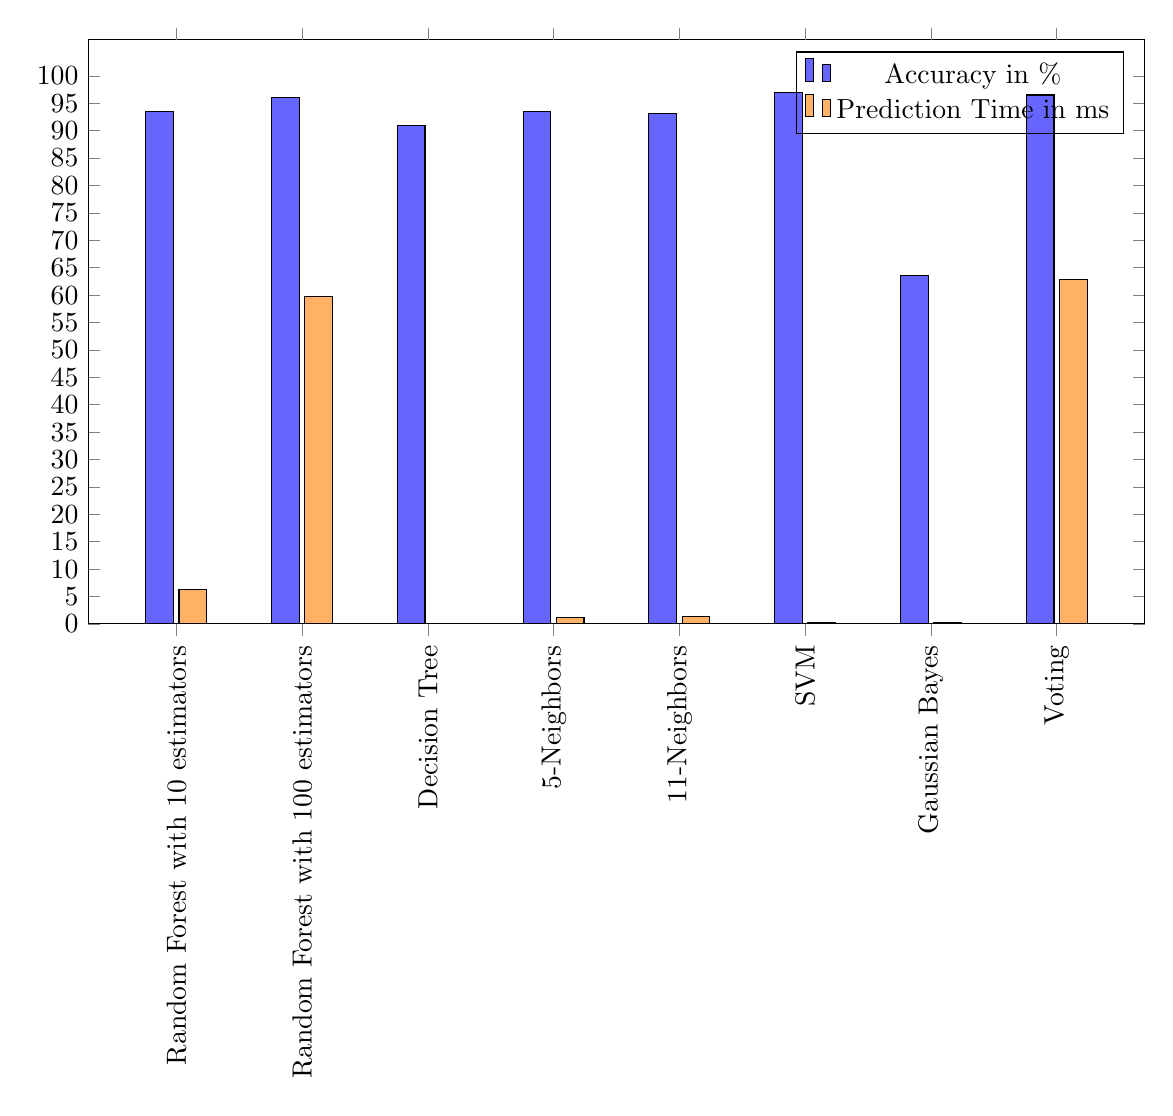
\begin{tikzpicture}
\begin{axis}[
    title = {},
    width=15cm,
	ymin=0,
    height=9cm,
    xtick=\empty,
    ytick={0,5,...,100},
    extra x ticks={1,...,8},
    extra x tick labels={%
		Random Forest with 10 estimators,
        Random Forest with 100 estimators,
        Decision Tree,
        5-Neighbors,
        11-Neighbors,
        SVM,
        Gaussian Bayes,
        Voting    
    },
    extra x tick style={
           grid=none,
           tick label style={rotate=90} % <-- this is added
           },
    legend style={fill=none},
    ybar
    ]

\addplot[
    fill=blue!60,
    draw=black,
    point meta=y,
    every node near coord/.style={inner ysep=5pt}
] 
table [y] {
x   y      label
1   93.5   1
2   96   2
3   91   3
4   93.5   4 
5   93.1   5 
6   96.9   6
7   63.5   7 
8   96.5   8
};

\addplot[
    fill=orange!60,
    draw=black,
    point meta=y,
    every node near coord/.style={inner ysep=5pt}
] 
table [y] {
x   y      label
1   6.3   1
2   59.8   2
3   0.1   3
4   1.1   4 
5   1.3   5 
6   0.2   6
7   0.3   7 
8   62.9   8
};

\legend{Accuracy in \%,Prediction Time in ms}
\draw ({rel axis cs:0,0}|-{axis cs:0,0}) -- ({rel axis cs:1,0}|-{axis cs:0,0});
\end{axis}
\end{tikzpicture}
\caption{Leave one out}\label{fig:loo}
\end{figure}

The K-Neighbors classifier follows a differnet approach. Simply put, training data is mapped into a coordinate system. Input data is then mapped the same way and classified by checking the K nearest training data points in that coordinate system relative to the input data. Whatever gesture the majority of these K neighbors is assigned to is the predicted gesture of our input. In our case K was five or eleven. Considering just 5 neighbors showed off to be the better solution and compares very vell to our Random Forest classifier with 100 estimators: The K-neighbors classifier performs about 2-3\% worse and has a higher standard deviation equal to 13\% in precision, accuracy and recall instead of 10\% - 12\%.

Having examined those common classifiers we combined the Random Forest classifier with 100 estimators and 5-Neighbors classifier as estimators into a Voting classifier. The Voting classifier passes input data to all its estimators and makes its decision based on their averaged predicted gesture probabilites. Tests revealed that giving the Random Forest predictions twice the weight of the 5-Neighbors predictions while using soft voting increases the accuracy and recall of our Voting classifier to 95\% while slightly decreasing the standard deviation to 9-8\%. The weight determines in the case of soft voting, as we applied it, the weight of the gesture probabilities before averaging.

Yet, the Support Vector Machine (SVM) classifier still beats the Voting classifier: 96\% accuracy, precision and recall with a standard deviation of 5\% each are the main reasons why we would chose the SVM classifier for dashboard interaction. Since well-tuned features and improved data preprocessing are important for an efficient SVM classifier we were only able to reach these results in the final phase of our work. For that reason the SVM classifier may be examined in further research and is currently not used in our dashboard application.

In order to provide a convenient user experience, gestures need to be predicted fast enough during app usage. We measured the average prediction time for each classifier during our leave one out tests. As our data set consists of 480 samples we iterated 480 times over it and left out a different data set on each iteration. The left out data set was used for testing, the remaining 479 data sets were used for training. The results are presented in figure \ref{fig:loo}.

Although the Voting classifiers prediction time of sixtytwo milliseconds is the highest one it competes very vell against \cite{liu}; our achieved delay is about five times shorter and therefore proves itself appropriate for real world applications. We implemented the Voting classifier in the dashboard and got statisfying test results. One might notice that the 5-Neighbors classifier needs approximately one millisecond and still performs almost as well as the Random Forest classifier with 100 estimators. So the relatively large prediction time of the Voting classifier is mainly caused by the Random Forest classifier we applied to the classifier set. Overall, the longer prediction time pays off as an increase of 3\% in accuracy, precision and recall values. 
In contrast, the SVM classifier stands out with a prediction time of 0.2ms. As it also performs slightly better than the Voting classifier it is the option to choose for production use.


%% ==============
\chapter{Dashboard}
\label{ch:Dashboard}
%% ==============

The main goal of our seminar work was to implement a gesture recognition program with which we can reliably control applications like dashboards on the computer.
Therefore, we created a test dashboard with which we examined the usability of our program.
Just like the previously decribed scanner, the dashboard module is only used by the recognizer app.
It provides the user with a user interface showing charts and diagrams based on stock market data which can be modified by steering elements like a dropdown menu and radio buttons.
The main characteristic of the dashboard is that it can be controlled only with a few simple buttons.
This makes the steering with our gesture recognition program easier since we can use the python package “pyautogui” to translate recognized gestures into commands on our user interface.

We decided to use the swipe left and right gestures to select a value in a dropdown menu and we use a punch gesture to cycle through the available years in data since these commands felt relatively intuitive. 

Of course, this is just a simplified example of a dashboard with only a few features compared to what can be found in actual corporate dashboards which allow more sophisticated commands.
Nevertheless, our dashboard can be easily extended with further features by implementing more steering elements like slide bars or check buttons and by adding more recognizable gestures with which these elements can be controlled.  

\begin{figure}[htp]
\begin{center}
  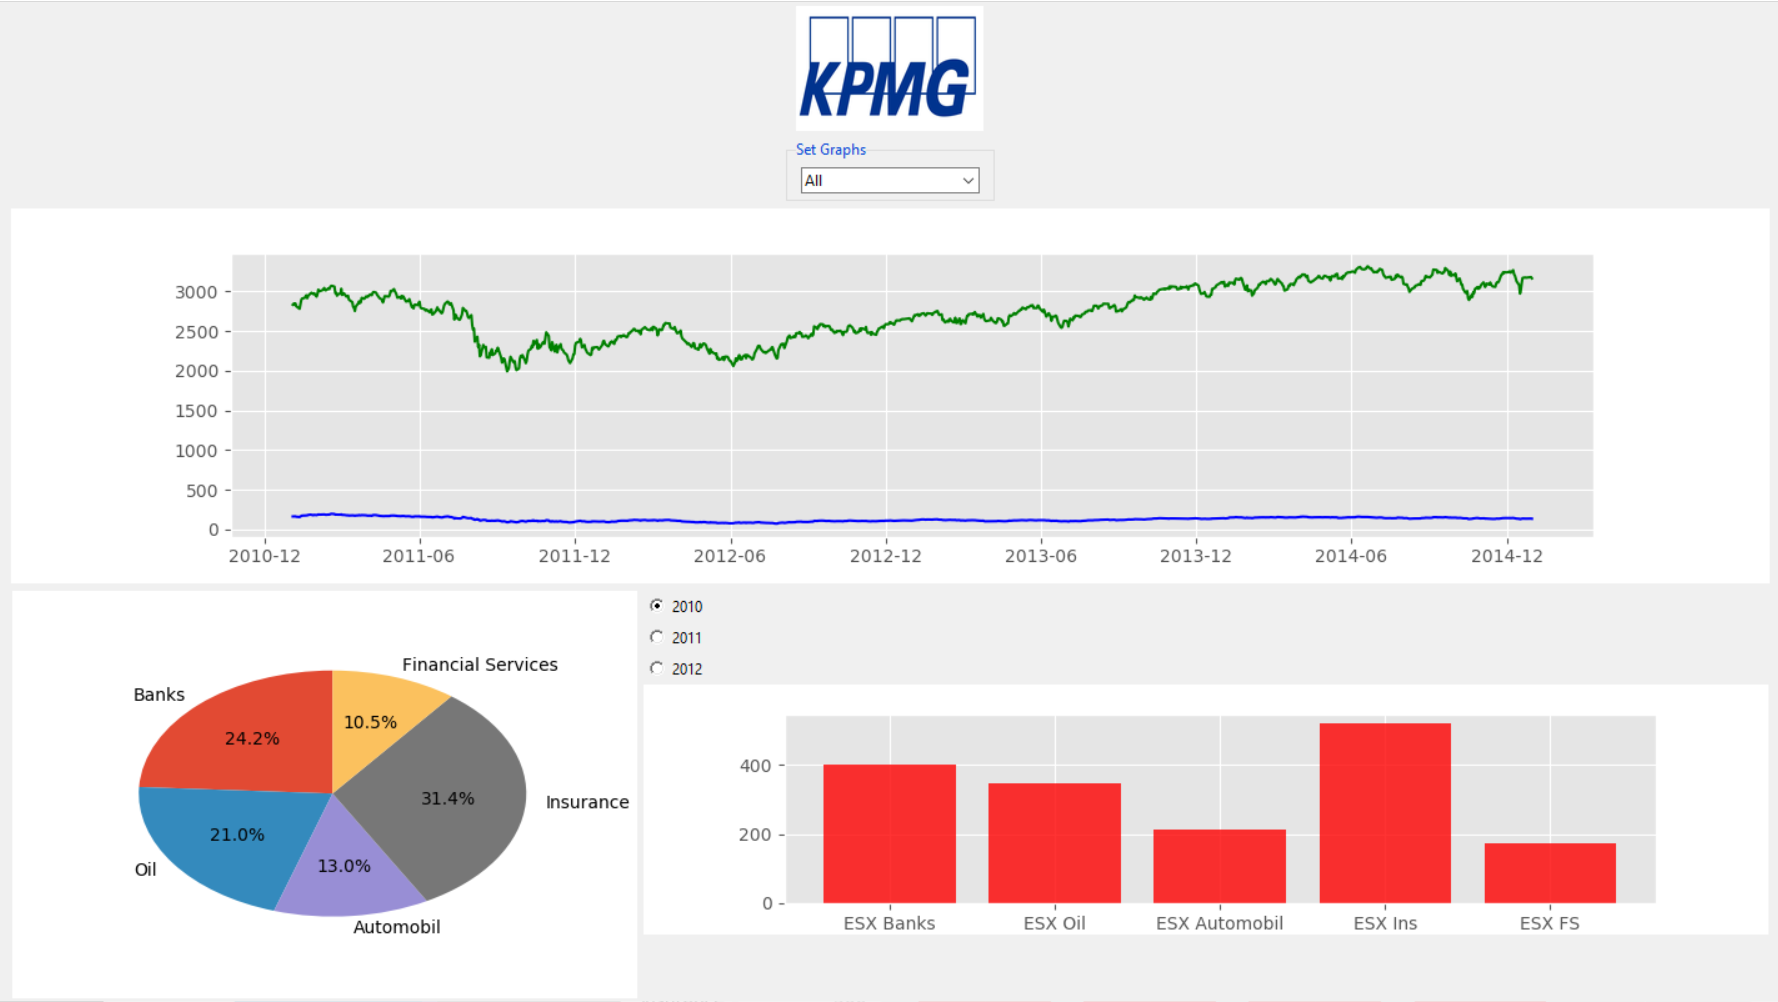
\includegraphics[width = \textwidth]{dashboard.png}
\caption{Our demo application front end}
\end{center}
\end{figure} 


%% ===========================
\chapter{Testing}
\label{ch:Tests}
%% ===========================

%% ===========================
\section{Functionality}
\label{ch:Results:sec:Functionality}
%% ===========================

In our tests, we noticed, that we can not fully reach the 95\% of precision that we theoretically achieved in our calculations.

The key factor why we don't reach this precision is the very low frequency of data given to us by the ThunderBoard.
We recieve only 5 data samples per seconds, our gestures are only half a second long.
This leads to the problem, that one data point can mix , for example, the fast movement to the left and the slow movement back to the right, so we only get one datapoint from two different movements.

We tried to make this better by recording more data, in different speeds and with slightly different movement, but the more data we use, the algorithms heavily get slower.

In the end we are very happy that we now recognize more than 80\% of the gestures and translate them into working dashboard commands.

\todo{More?}

%% ===========================
\section{Usability}
\label{ch:Results:sec:Usability}
%% ===========================

\todo{Usability tests with other people}

%% ===========================
\chapter{Results}
\label{ch:Results}
%% ===========================

In this seminar paper, we present a gesture recognition system for dashboard steering via a Thunderboard React. 
Core of this implementation are the machine learning algorithms which are used to classify the input data and to recognize the different gestures. 
We used several algorithms, like Random Forest, k-Nearest Neighbors, Support Vector Machine or a Voting classifier which we trained with overall 480 samples for four different gestures. 
Our experiments demonstrated that our implementation achieves an expected accuracy of 95\% with a delay of only 56 milliseconds by using a Voting classifier. 
Furthermore, we used the gesture recognition for controlling a dashboard that we created. 
In practice, over 80\% of the gestures could be recognized and translated correctly into dashboard commands, which is a decent result. 
\newline
We also investigated the usability of the gesture based dashboard steering. 
In experiments, we let participants use the gesture recognition on the dashboard and evaluate their experience \todo{..write some results of the usability test}
\newline
Nevertheless, our work exposes several extension opportunities. 
First of all, further recognizable gestures can be added in order to increase the usability of our implementation for industrial purposes. 
This would also allow the user to control a more sophisticated dashboard with more steering elements than the one used in our work.
Further gestures and a higher accuracy can be realized by utilizing data from the Hall sensor on the Thunderboard react, so that more features can be calculated as training data for the machine learning algorithm. 
Also, more sample data for the training of the algorithms is valuable, which was unfortunately not possible in this work due to the limited time that was available. 
Moreover, a combination of our work with tactile feedback devices can also be implemented in order to enhance a user’s dashboard experience even more. 



%% evaluation.tex
%%

%% ==================
\chapter{Results \& Conclusion}
\label{ch:Results}
%% ==================

\dots



%% ----------------
%% |   Appendix   |
%% ----------------
% IM Style: No additional blank page
% \cleardoublepage

%%% appendix.tex
%%

%% ==============================
%\chapter{Appendix}
%\label{ch:Appendix}
%% ==============================

\appendix

\iflanguage{english}
{\addchap{Appendix}}	% english style
{\addchap{Anhang}}	% german style


\section{First Appendix Section}
		\label{Anhang-Implementierung}
		
\setcounter{figure}{0}

\dots






%% --------------------
%% |   Bibliography   |
%% --------------------
\cleardoublepage
\phantomsection
\addcontentsline{toc}{chapter}{\bibname}

% IM Style
\iflanguage{english}
{\bibliographystyle{apacite}}	% english style
{\bibliographystyle{apacite}}	% german style

%

% Informatik-Style
%\iflanguage{english}
%{\bibliographystyle{IEEEtranSA}}	% english style
%{\bibliographystyle{babalpha-fl}}	% german style
												  
% Use IEEEtran for numeric references
%\bibliographystyle{IEEEtranSA})

\bibliography{thesis}


\end{document}
